\section{Spin flipping and Mossbauer}

In Mossbauer spectroscopy the nuclear decay of $Cobalt^{57}$ to $Fe^{57}$ is often used: $Co^{57} \Rightarrow Fe^{57}$.
A good introduction is by prof Guetlich \cite{Guetlich}.

Figure~\vref{fig:nuclear_decay_scheme_57fe_mossbauer} shows the different energy levels and the energies of the emitted photons.


\begin{figure}[!ht]
    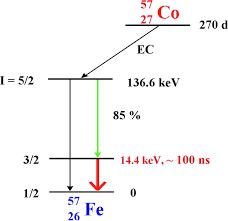
\includegraphics{nuclear_decay_scheme_57fe_mossbauer.png}
    \caption{Nuclear decay scheme 57fe Mossbauer\label{fig:nuclear_decay_scheme_57fe_mossbauer}}
    
\end{figure}


\includepdf[ pages={12,40,82,90} , nup=2x2, frame]{./bib/Cited_webpages_copy/Moessbauer_Lectures.pdf}


$^{57}Co$ has a spin of $\sfrac{7}{2}$, so in our model it has at least 7 long ornac-sticks with three nucleids. These are oriented in about the same direction to create the magnetic moment.
$Co^{57}$ has 27 protons and 30 neutrons, so of the 7  long ornac-sticks three are from the surplus of neutrons, so thrice $1p+2n$, these are Tritium sticks. 

The other four are made up by a combination of twice $2p+1n$ and twice $1p+2n$. So a total of two Hetrium sticks and five Tritium sticks.

\paragraph{}
$Co^{57}$  decays by electron capture: one of the Hetrium sticks captures the electron and transforms into a Tritium stick. The transform from hetrium to tritium lets the magnetic field flip in orientation. So $Fe^{57}$ in its first state has a spin of $I = \sfrac{5}{2}$.

So we can conclude that $Fe^{57}$ has at least 7 long ornac-sticks of which one is a Hetrium stick.
This decays quickly into $Fe^{57}$ $\sfrac{3}{2}$. This happens by a rearrangment of the long ornac-sticks: one of them flips direction so it cancels the magnetic field of one other stick.

\paragraph{}
Another thing is that there is the same number of long ornac-sticks in $Co^{57}$ and $Fe^{57}$.
Both have 18 short ornac-sticks made of Deuterium sticks. 

\begin{center}
  \begin{tabular}{ | l || c | r |}
    \hline
     & $Co^{57}$ & $Fe^{57}$ \\ \hline\hline 
    Deuterium & 18 & 18 \\ \hline 
    Tritium & 5 & 6 \\ \hline 
    Hetrium & 2 & 1 \\ \hline 
    Spin I & $\sfrac{7}{2}$ & $\sfrac{1}{2}$ \\ \hline 
    Magnetic Mo & $4.7\mu$ & $0.09\mu$ \\ \hline 
    \hline
  \end{tabular}
\end{center}
\paragraph{}
Let's put it in a table and take a step back.\\
Why is the magnetic moment a factor 50 different,\\ 
while the spin is a factor 7?

\paragraph{}
If you would just look up $Fe^{57}$ and found spin $I = \sfrac{1}{2}$, we might just think: 
\begin{quotation}
Ok, there is spin $\sfrac{1}{2}$.\\
So, there is one stick with three nucleids.\\
And why is the magnetic moment so small.
\end{quotation}

\paragraph{}
But now we think:
\begin{quotation}
OK, we know it started with seven long odd sticks.\\
All those fields cancel eachother almost,\\
When they are randomly aligned.\\
So we end up with a small net magnetic moment.
\end{quotation}




